\documentclass{article}
\usepackage[top=0.75in, bottom=0.75in, left=1.25in, right=1in]{geometry} %formatage%
\usepackage{amsmath} %pour utiliser des maths de base%
\usepackage{amssymb} %pour faire \mathcal{}=>des lettres ''cursives''%
\usepackage{amsthm} % La petite boîte de fin de preuve
\usepackage{graphicx} %pour importer des images...http://www.tex.ac.uk/cgi-bin/texfaq2html?label=figurehere%
\usepackage{titlesec} %automatique, pour faire des sous-titres moins laids%
%\usepackage{cancel}
\usepackage[procnames]{listings}
\usepackage[utf8]{inputenc} 
\usepackage[T1]{fontenc}        %http://tex.stackexchange.com/questions/11897/draw-a-diagonal-arrow-across-an-expression-in-a-formula-to-show-that-it-vanishes%
\usepackage[frenchb]{babel}
\usepackage{xcolor}
\usepackage[squaren]{SIunits}
\usepackage{subcaption} % Avoir plusieurs sous-figures (graphiques) dans une figures et pouvoire les étiqueter
\usepackage{color}
\usepackage{lipsum}
\usepackage{caption}
\usepackage{wasysym} 
\usepackage{braket}
\usepackage{mathtools}
\usepackage{mathrsfs} % Faire le symbole de la transformée de Laplace
\usepackage{bbm}
\usepackage{array}
\usepackage{diagbox}        
\usepackage{dsfont} % Faire des belles indicatrices                         %diagonale dans les tableaux
\usepackage{float}%placer les tableaux et images où tu veux
\usepackage{listings}
\usepackage[utf8]{inputenc}
\usepackage{comment}
\usepackage{pst-node}
\usepackage{fancyvrb} % Les varbatims gardent l'indentation
\usepackage{enumitem}
\usepackage{breakcites} % Faire en sorte que les citations ne sortent pas dans la marge
\usepackage{graphicx} % Insérer des graphiques
\usepackage{pgfplots}
\pgfplotsset{width=10cm, compat=1.9}
%\usetikzlibrary{patterns,decorations.pathreplacing}
%
%\newcommand{\tikzmark}[2]{%
%	\tikz[remember picture,baseline=(#1.base)]
%	\node[circle,red,draw,text=black,anchor=center,inner sep=1pt] (#1) {#2};}
%\newcommand{\tikzmarkk}[2]{%
%	\tikz[remember picture,baseline=(#1.base)]
%	\node (#1) {#2};}


%\setcounter{secnumdepth}{0} % sections are level 1

\newtheorem{lemme}{Lemme}
\newtheorem{preuve}{Preuve}
\newtheorem{code}{Code informatique}
\newtheorem{exemple}{Exemple}
\newtheorem{scenario}{Scénario}


\begin{document}
	\renewcommand{\tablename}{Tableau}
	\renewcommand{\figurename}{Illustration}
	
	\begin{titlepage}
		\centering % Centre everything on the title page
		
		\scshape % Use small caps for all text on the title page
		
		\vspace*{7\baselineskip} % White space at the top of the page
		
		%------------------------------------------------
		%	Title
		%------------------------------------------------
		
		\rule{\textwidth}{1.6pt}\vspace*{-\baselineskip}\vspace*{2pt} % Thick horizontal rule
		\rule{\textwidth}{0.4pt} % Thin horizontal rule
		
		\vspace{0.75\baselineskip} % Whitespace above the title
		{\LARGE Résumé de ce qui a été fait depuis votre départ. \\} % Title
		\vspace{0.75\baselineskip} % Whitespace below the title
		
		\rule{\textwidth}{0.4pt}\vspace*{-\baselineskip}\vspace{3.2pt} % Thin horizontal rule
		\rule{\textwidth}{1.6pt} % Thick horizontal rule
		
		\vspace{3\baselineskip} % Whitespace after the title block
		
		%------------------------------------------------
		%	Subtitle
		%------------------------------------------------
		{\scshape\Large Sous la supervision de \\Étienne Marceau\\} % Editor list
		
		\vspace*{3\baselineskip}
		
		  % Subtitle or further description
		
		\vspace*{3\baselineskip} % Whitespace under the subtitle
		
		%------------------------------------------------
		%	Editor(s)
		%------------------------------------------------
		
		Préparé par
		
		\vspace{0.5\baselineskip} % Whitespace before the editors
		
		{\scshape\Large Alexandre Lepage, \\
			Diamilatou N'diaye, \\} % Editor list
		
		\vspace*{5\baselineskip}
		
		le $1^{er}$août 2019
		
		\vspace{0.5\baselineskip} % Whitespace below the editor list
		
		\vfill % Whitespace between editor names and publisher logo
		
		%------------------------------------------------
		%	Publisher
		%------------------------------------------------
		
		
\includegraphics[height=1.2cm]{UL_P.pdf}\\
		
		Faculté des sciences et de génie\\
		École d'actuariat\\
		Université Laval\\     
	\end{titlepage}

	\pagenumbering{Roman} % Pagination en chiffres romains
	\setcounter{page}{0} 
	
	\newpage
	\strut % Page blanche
	\newpage
	
	\tableofcontents
	\renewcommand{\listfigurename}{Liste des illustrations}
	\listoffigures
	\newpage
	
	\pagenumbering{arabic} % Pagination en chiffres normaux
	\setcounter{page}{1}
	
	\section{Estimation de paramètres avec une copule archimédienne à hautes dimensions.}
	\label{sect_vrais_haute_dim}
	
	Dans les étapes précédentes du projet, nous avons trouvé que la méthode du maximum de vraisemblance complète donnait d'excellents résultats pour estimer les paramètres d'un échantillon simulé. Cependant, le principal désavantage de cette méthode sont les temps de dérivation et d'optimisation numérique. Nous avons donc testé la méthode du maximum de vraisemblance composite. Cette dernière estimait précisément les paramètres des lois marginales ainsi que le paramètre de dépendance de la loi mère de la copule archimédienne hiérarchique. Par contre, lorsque venait le temps de calculer le paramètre de la loi enfant, nous étions confronté au même problème qu'avec la méthode complète puisque les montants de sinistres sont tous regroupés ensemble dans une même copule archimédienne. Dans un contexte d'assurance, il n'est pas impossible de voir un nombre de sinistre supérieur à 10. Il faut donc trouver une façon alternative d'estimer le paramètre de dépendance de la loi enfant. Plusieurs solutions sont présentées dans \cite{hofert2013ArchimedeanHighDimension}. \\
	
	Pour débuter, la méthode des moments en inversant le tau de Kendall n'est pas une solution envisageable puisque, lorsque l'on utilise cette méthode, l'estimation du paramètre de dépendance de la loi enfant est fortement influencée par le niveau de dépendance induit par la loi mère comme le démontre l'illustration \ref{graph_alpha1_fct_de_alpha0}.
	
	\begin{figure}[ht]
		\centering
		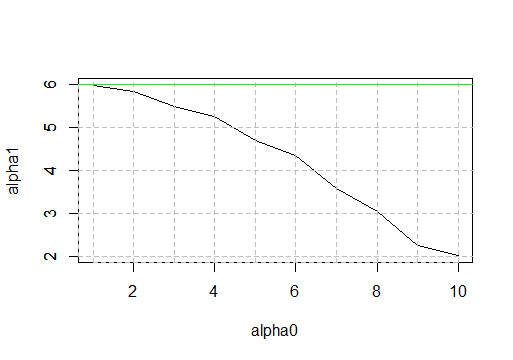
\includegraphics[height=7cm]{graph/alpha1_fct_de_alpha0.png}
		\caption[Influence de $\alpha_{0}$ dans l'estimation de $\alpha_1$ par inversion du tau de Kendall]{Influence de $\alpha_{0}$ dans l'estimation de $\alpha_1$ par inversion du tau de Kendall : 
			Cette illustration est générée en simulant $10 \times 10\,000$ observations du modèle collectif du risque présenté dans \cite{Itre5} pour $\alpha_{0} = 1,\dots, 10$, $\alpha_{1}$ demeure constant à $6$ et la copule est logarithmique-logarithmique. La ligne verte correspond au vrai paramètre $\alpha_1$ définit pour les simulations.}
		\label{graph_alpha1_fct_de_alpha0}
	\end{figure}

	De son côté, Diamilatou a trouvé \eqref{eq_densite_archi_high_dim} afin de pouvoir dériver la copule en plusieurs étapes afin de réduire le temps de dérivation. D'ailleurs, il se trouve que \eqref{eq_densite_archi_high_dim} correspond à l'équation (9) de \cite{hofert2013ArchimedeanHighDimension}.
	
	\begin{equation} \label{eq_densite_archi_high_dim}
		c(\textbf{u}) = \psi^{(d)} \left(\sum_{j=1}^{d} \psi^{-1}(u_j) \right) \times \prod_{j=1}^{d} (\psi^{-1})'(u_j)
	\end{equation}
	
	Nous avons donc programmé cette équation. Celle-ci donne la possibilité d'imbriquer la fonction \texttt{R sapply} dans l'expression de la dérivée; ce qui permet d'augmenter l'efficacité des calculs en réduisant les temps d'optimisation numérique pour estimer les paramètres. Cependant le temps de dérivation demeure problématique puisqu'il faut toujours dériver $d$ fois la fonction génératrice $\psi(t) = \mathscr{L}_{\Theta}(t) = \mathcal{P}_{M} \circ \mathscr{L}_B(t)$. Ce qui nous limite, de façon général, à 5 dérivées.\\
	
	Il reste donc la solution de la dérivation numérique proposée par \cite{hofert2013ArchimedeanHighDimension}, à la page 38 où il estime $\psi^{(d)}$, soit en évaluant numériquement \eqref{eq_estim_derive_avec_integrale} ou en simulant avec \eqref{eq_approx_deriv_MC}.
	
	\begin{equation}\label{eq_estim_derive_avec_integrale}
		(-1)^d \psi^{(d)}(t) = \int_{0}^{\infty} \theta^d e^{-\theta t} \textrm{d}F_\Theta(\theta) = \mathbb{E}\left[\theta^d e^{-\theta t} \right],\; t \in(0,\infty)
	\end{equation}
	 
	\begin{equation}\label{eq_approx_deriv_MC}
		(-1)^d \psi^{(d)}(t) \approx \frac{1}{m} \sum_{k=1}^{m} \theta_{k}^{d} e^{-\theta_{k}t}),\; t \in(0,\infty),
	\end{equation}
	
	où $\theta_k \sim F_{\Theta}, k \in \{1,...,m\}$, $m$ est le nombre de simulations nécessaires à l'estimation de la dérivée. Il doit être raisonnablement grand (ex: $10\,000$). Cependant, lorsque l'on regarde \eqref{eq_estim_derive_avec_integrale}, on voit qu'il faut connaître $F_{\Theta}$. À ce stade, nous n'avons pas tenté de trouver les fonctions de répartition de $\Theta$ pour chacune des lois. Cependant, cela ne devrait pas être trop difficile et pourrait nous permettre de résoudre le problème de temps de dérivation. Par contre, autant pour l'intégration numérique que pour la simulation Monte Carlo, cette méthode augmenterait considérablement les temps de calcul. À ce moment-ci, l'utilisation d'un \textit{GPU} pourrait permettre d'obtenir des temps de calcul raisonnables.\\
	
	\section{Revue de littérature sur le modèle collectif du risque avec structure de dépendance.} 
	\label{sect_revue_litterature}
	Après avoir essayé les solutions présentées dans la section \ref{sect_vrais_haute_dim}, nous avons lu plusieurs articles pour prendre du recul et voir ce qui se faisait dans la littérature au sujet du modèle collectif du risque avec structure de dépendance. Pour débuter, le tableau \ref{graph_revue_litterature} permet de comparer, d'un premier coup d'œil, les différents articles. Par la suite, un court résumé est fait pour chacun d'eux.
	
	\begin{figure}[ht]
		\centering
		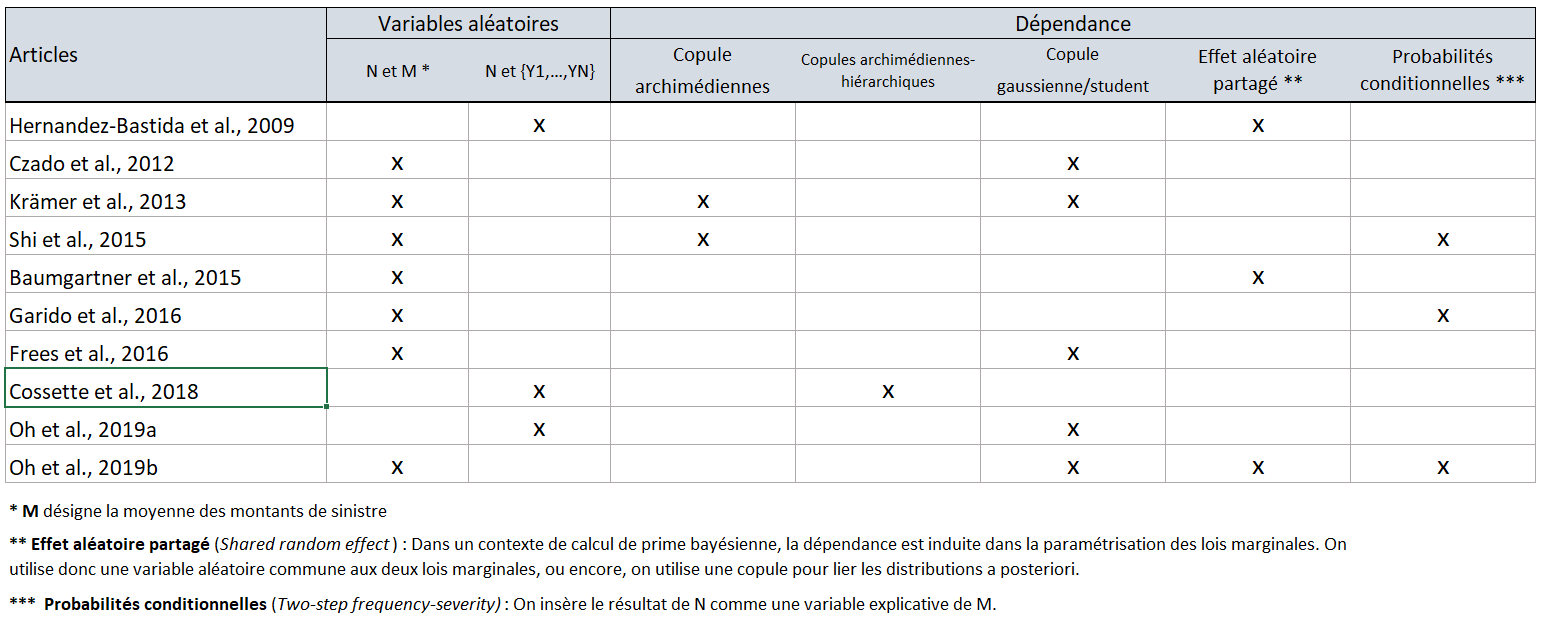
\includegraphics[height=6.5cm]{graph/Tableau_revue.PNG}
		\caption{Classification des articles lus sur le modèle collectif du risque avec dépendance.}
		\label{graph_revue_litterature}
	\end{figure}

	\subsection{Modèle de probabilités conditionnelles (\textit{Two-steps frequency-severity model})}
	Les modèles de probabilités conditionnelles ou, communément appelés dans la littérature, \textit{The two-steps frequency-severity models} sont, de loin, les modèles les plus simples autant dans l'interprétation que dans la paramétrisation puisqu'ils se résument simplement à utiliser la réalisation de la v.a. $N$ comme une variable explicative du modèle linéaire généralisé (glm) de la v.a. $M$, où $M=\frac{1}{n}\sum_{j=1}^{n} Y_j$. \\
	
	D'une part, \cite{garrido2016generalized} explique comment cette approche est mise en place. D'autres part, \cite{shi2015Dependant} compare ce type de modèle avec celui utilisant des copules. Finalement, dans ce dernier article, l'auteur vient à la conclusion que les modèles utilisant des copules sont beaucoup plus précis du fait qu'il permette d'induire des relations de dépendance autres que linéaire et peuvent donc mieux s'adapter aux données.

	\subsection{Copules}
	En ce qui a trait aux copules, \cite{kramer2013total} explique vraiment bien comment créer un modèle basé sur des copules. Il propose également une méthodologie pour choisir la copule à adopter en fonction du ratio de vraisemblance. Par la suite, \cite{czado2012mixed} propose une méthode alternative à la maximisation de la vraisemblance standard pour estimer les paramètres du modèle. Cette méthode se fonde sur le score de Fisher et est utilisée par la fonction \texttt{R glm} pour estimer les paramètres des modèles linéaires généralisés. L'avantage de cette approche est qu'elle permet d'estimer un très grand quantité de paramètres à la fois en utilisant un nombre d'itération minimal.\\
	
	Par la suite, \cite{oh2019copula} présente une méthode alternative à \cite{Itre5} pour modéliser la dépendance entre $N$ et $\{Y_1,\dots,Y_n\}$ en construisant une copule gaussienne avec une matrice de corrélation utilisant deux paramètres. Cette méthode est intéressante du fait qu'elle ne nécessite pas un long processus de dérivation pour trouver la densité de la copule. De plus, il est possible de travailler avec des réalisations de $N$ qui peuvent prendre des valeurs élevées. Dans l'étude de cas présenté dans l'article, il y avait jusqu'à 12 sinistres pour un même assuré.% Par contre, dans la littérature, il est fait mention que la copule gaussienne est excellente pour modéliser des niveaux de dépendance faibles à modérés, mais qu'elle ne performe pas bien lorsque la dépendance est élevée. Il faut donc faire attention à cet aspect avec ce modèle. 
	

	\subsection{L'effet aléatoire partagé (\textit{Shared random effect})}
	La méthode de l'effet aléatoire partagé repose sur le calcul de la prime d'assurance en utilisant l'approche de crédibilité bayésienne. Se faisant, on peut induire de la dépendance entre les v.a. de fréquence et de sévérité à l'aide de leurs classes de risques respectives que l'on peut dénoter $\Theta_N$ et $\Theta_Y$. Pour ce qui est de l'estimation des paramètres il s'agit d'avoir recours à la méthode de Monte Carlo pour simuler des chaînes de Markov. Dans la littérature, cela est appelé la méthode MCMC (Voir \cite{brooks2011handbook} et \cite{roberts2004general}).\\
	
	Dans \cite{hernandez2009net}, on utilise la famille de distributions bivariées de Samarnov-Lee, dont la copule FGM fait partie, pour créer une structure de dépendance entre $\Theta_N$ et $\Theta_Y$. De cette façon, les réalisations de $Y$ sont liées entre elles puisqu'elles partagent la même classe de risque et un lien de dépendance est créé entre les v.a. $N$ et $Y$ grâce à la copule qui lie leurs distributions a posteriori. De plus, l'avantage d'induire la dépendance à travers la classes de risque permet de présumer l'indépendance des montants de sinistre conditionnellement à cette classe. Ainsi, on peut utiliser la relation $\mathbb{E}[S|\Theta_N=\theta_N, \Theta_Y=\theta_Y]  = \mathbb{E}[N|\Theta_N=\theta_N] \times \mathbb{E}[Y|\Theta_Y=\theta_Y]$ sans perdre de précision en agrégeant les réalisation de $Y$.\\
	
	Par la suite, \cite{baumgartner2015bayesian} présente une façon alternative d'utiliser l'effet aléatoire partagé. En effet, dans l'article, plutôt que d'utiliser une copule pour créer la relation entre $N$ et $Y$, on ajoute une variable explicative commune aux modèles linéaires généralisés des distributions marginales qui servira exclusivement à insérer de la dépendance entre les variables aléatoires. Cette façon de faire permet une simplification du modèle présenté par \cite{hernandez2009net} de même que la possibilité d'avoir plusieurs niveaux de dépendance différents selon la classe de risque. Finalement, lors d'une analyse de cas, l'auteur compare son modèle à celui présenté par \cite{kramer2013total} pour venir à la conclusion que le sien était plus précis et plus flexible.\\
	
	En ce qui a trait à \cite{oh2019implementation}, non seulement on reprend un modèle similaire à \cite{hernandez2009net} dans le sens où on utilise une copule gaussienne pour créer un lien de dépendance entre les classes de risque de $N$ et $M$, mais, en plus, on ajoute la réalisation de $N$ comme variable explicative dans le glm de la distribution a priori de $M$. Autrement dit, l'auteur a combiné deux approches pour intégrer une structure de dépendance entre les composantes de son modèle. Est-ce que cette méthode accorde trop de poids à la dépendance ? Il faudrait faire le test en comparant avec l'approche de \cite{hernandez2009net} ou de \cite{baumgartner2015bayesian}.
	
	\section{Conclusion}
	Dans l'ensemble, les modèles avec effet aléatoire partagé semblent constituer l'approche la plus prometteuse en termes de précision. Cependant, elle est aussi la plus compliquée à mettre en place. Le modèle proposé dans \cite{Itre5} offre une approche alternative aux modèles traditionnels impliquant des copules du fait qu'elle considère un lien de dépendance possible entre les réalisations de $Y$. Cependant, cette approche ne considère pas la possibilité que la dépendance peut varier selon les groupes de risques des assurés et elle rencontre des problèmes dans l'estimation des paramètres lorsque la v.a. $N$ peut prendre de grandes valeurs. Pour cette raison, il semblerait qu'il serait préférable d'adopter un modèle basé sur l'effet aléatoire partagé. Il reste cependant à voir si cette approche peut aussi bien servir à calculer la réserve actuarielle qu'elle le fait pour déterminer les primes ou bien si elle est trop complexe à mettre en place; auquel cas, l'approche proposé par \cite{oh2019copula} constituerait une alternative intéressante.
	
	
	\newpage
	\bibliography{BibRRT.bib}
	\bibliographystyle{apalike}
\end{document}